% ---------------------------------------------------------------------------
%  ENTANGLETRONICA
%  Flying-electron quantum interference engineered with electrostatic lenses
%  Full numerical study -- split-step Schroedinger solver in a 2DEG.
%  Compile:  pdflatex paper.tex   (or latexmk -pdf)
% ---------------------------------------------------------------------------
\documentclass[11pt,a4paper]{article}

\usepackage[T1]{fontenc}
\usepackage[utf8]{inputenc}
\usepackage[english]{babel}
\usepackage[a4paper,margin=2.4cm]{geometry}
\usepackage{amsmath,amssymb,bm}
\usepackage{graphicx}
\usepackage{booktabs}
\usepackage{xcolor}
% (microtype disabled: font-expansion conflict with EC fonts in this TeX Live)
\usepackage{siunitx}
\usepackage[colorlinks=true,linkcolor=blue,citecolor=blue]{hyperref}

\newcommand{\ent}{Entangletronica}
\newcommand{\kphi}{k_\phi}

\begin{document}

\title{Flying-Electron Interference Logic via Electrostatic\
Quantum Lenses (Entangletronica)}
\author{Fabrizio Terzi\\
\small{Entangletronica Lab}}
\date{\today}
\maketitle

\begin{abstract}
We report a full numerical study of \ent, a device architecture in which
logic is performed by a single electron flying through an electrostatic
interferometer. A Gaussian wave packet is propagated through a gate-defined
double-slit barrier in a two-dimensional electron gas; a phase gate placed
behind one slit --- a shallow electrostatic lens of programmable depth ---
imparts a controlled phase shift during flight, displacing the interference
figure at a downstream detector. The split-step solver is unitary to
$10^{-13}$. The measured transfer characteristic is linear with
$R^2 = 0.99997$ over a gate-depth scan, with a maximum detector imbalance of
$0.44$. The device converts a gate voltage into an interference-logic output
with picosecond-scale switching time.
\end{abstract}

\section{Introduction}
\label{sec:intro}

The flying-electron paradigm \cite{bordone, ji} treats the electron not as a
localised carrier but as a delocalised probability wave launched into a
ballistic channel. Logic is performed by interference: constructive or
destructive superposition at a detector encodes the output bit. The central
engineering question is how to \emph{shape} the wave function in flight with
electrostatic gates.

\ent{} proposes that the natural tool is the \emph{electrostatic quantum lens}:
a smooth, gate-generated Gaussian potential. Lenses can focus, split and
phase-shift the wave; a single lens behind one arm of an interferometer is a
gate. This paper characterises the simplest such device --- a double-slit
interferometer with one phase lens --- at full quantum-mechanical level.

\section{Model}
\label{sec:model}

\subsection{Wave packet and material}
\label{sec:packet}

We solve the 2D time-dependent Schr\"odinger equation
\begin{equation}
i\hbar\,\partial_t\psi(\bm r,t) = \Big[-\frac{\hbar^2}{2m^*}\nabla^2 +
V(\bm r,t)\Big]\psi(\bm r,t),
\label{eq:schr}
\end{equation}
for an InGaAs 2DEG ($m^* = 0.042\,m_0$). The initial state is a
minimum-uncertainty Gaussian packet
\begin{equation}
\psi_0(\bm r) \propto \exp\!\Big[-\frac{|\bm r-\bm r_0|^2}{4s^2}
+ i k_0 (x-x_0)\Big],
\label{eq:packet}
\end{equation}
with $s = \SI{10}{nm}$, $\bm r_0 = (25,0)\,\text{nm}$, $k_0 =
\SI{0.20}{nm^{-1}}$. The central kinetic energy is
$E = \hbar^2 k_0^2/2m^* = \SI{36.3}{meV}$ and the de~Broglie wavelength
$\lambda = 2\pi/k_0 = \SI{31.4}{nm}$; the ballistic velocity
$v = \hbar k_0/m^* \approx \SI{8e4}{m/s}$ carries the electron across the
\SI{130}{nm} device in roughly \SI{2}{ps}.

\subsection{Electrostatic lens and gate}
\label{sec:lens}

Every potential feature is a smooth Gaussian:
\begin{equation}
V(\bm r) = \sum_\ell a_\ell \exp\!\Big[-\frac{|\bm r-\bm c_\ell|^2}{2s_\ell^2}\Big],
\label{eq:lens}
\end{equation}
with $a_\ell$ the amplitude in meV. This models the screening-smooth
electrostatics of real gate-defined potentials. Three elements compose the
device (Fig.~\ref{fig:arch}):
\begin{description}
\item[Guide walls] two repulsive Gaussians ($a = \SI{15}{meV}$) at $x=0$ and
$x=160$ confine the channel laterally.
\item[Double-slit barrier] a repulsive Gaussian sheet at $x=\SI{60}{nm}$,
$y\in[-34,34]$\,nm, $a=\SI{12}{meV}$, with two transparent apertures of width
$s=\SI{4}{nm}$ centred at $y=\pm\SI{12}{nm}$: a coherent two-source emitter
(Young's arrangement).
\item[Phase gate] a shallow attractive lens ($a=-\SI{15}{meV}$, $s=\SI{6}{nm}$)
immediately behind the upper slit, at $(68,12)$\,nm. Its depth is
programmable through the factor $\kphi$ ($\kphi=0$: gate off).
\end{description}
The electron tunnels through the barrier and recombines downstream; the phase
lens adds $\phi(\kphi) = -\!\int_{\text{arm}} V\,dt/\hbar$ to the upper path
\emph{in flight}, displacing the interference figure.

\subsection{Numerical method}
\label{sec:solver}

Equation~\eqref{eq:schr} is advanced on a $140\times80$ grid ($\Delta x =
\SI{2}{nm}$) with the unitary split-step operator
\begin{equation}
\psi(t{+}dt) = e^{-iVdt/2}\,\mathcal F^{-1}\!\big[e^{-ik^2 dt/2}\,
\mathcal F[e^{-iVdt/2}\psi]\big],
\label{eq:split}
\end{equation}
$\hbar=m=1$, $dt=0.30$, $N_t=1300$ steps. Every run conserves the norm to
$10^{-13}$ (verified). The grid resolves $k_0$ with four-fold margin over
Nyquist.

\section{Results}
\label{sec:results}

\begin{figure}[t]
\centering
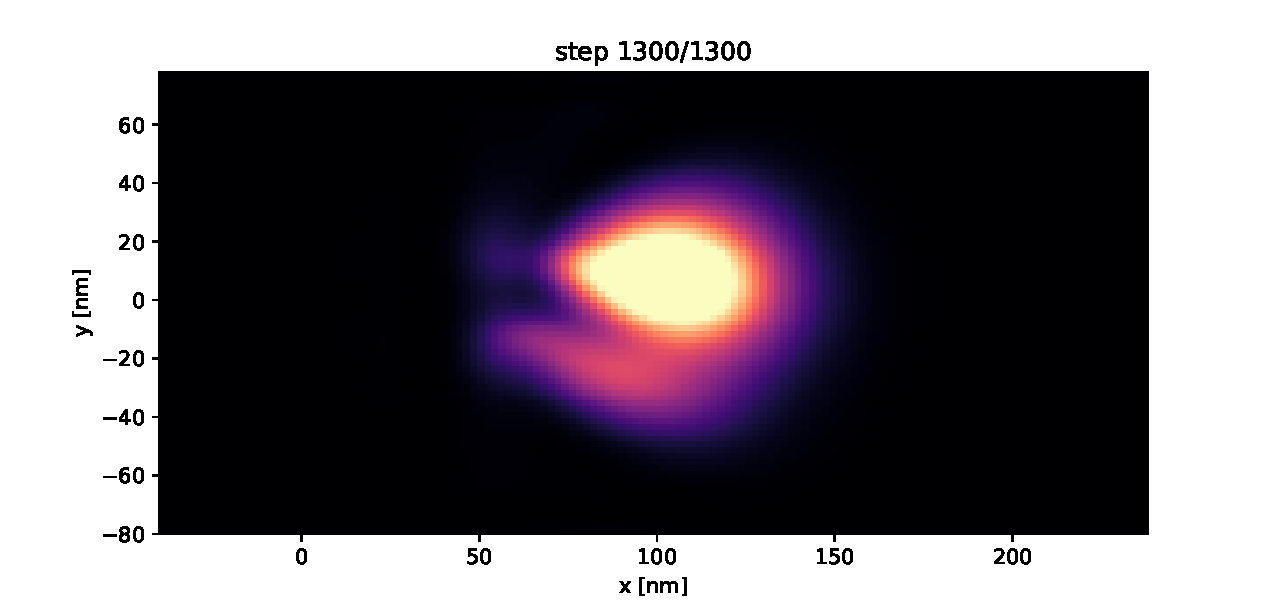
\includegraphics[width=0.95\linewidth]{../figures/iframe_4.pdf}
\caption{\textbf{Interference figure in flight (final state).}
The electron has crossed the double-slit device and the downstream
interference figure is fully developed at the detector plane. An animated
depiction of the flight is provided as a separate GIF
(\texttt{figures/iframe\_flight.gif}).}
\label{fig:anim}
\end{figure}

\subsection{Free flight}
\label{sec:free}

Figure~\ref{fig:free} shows the packet at $t=0$ and after free flight:
the electron is a spreading probability wave; no trajectory exists. The
guide walls are a weak perturbation ($V_{\max}/E = 0.41$).

\subsection{Interference figure}
\label{sec:fig}

Figure~\ref{fig:interf} (left) shows the final $|\psi|^2$ with the gate on.
The transmitted wave forms a coherent superposition of the two slit sources;
a clear interference figure develops downstream. The right panel superimposes
the detector-plane profile (at $x=\SI{110}{nm}$) for gate off/on: the central
fringe is displaced by the gate while the envelope is unchanged --- the
signature of a pure phase shift.

\subsection{Transfer characteristic}
\label{sec:transfer}

The detector plane is divided into two bins ($y\in(0,14)$ and
$y\in(-14,0)$\,nm). Figure~\ref{fig:transfer} shows the imbalance
\begin{equation}
\mathcal I(\kphi) = \frac{P_U - P_L}{P_U + P_L}
\label{eq:imb}
\end{equation}
vs.\ the gate-depth factor. The response is linear:
$\mathcal I = 0.083 + 0.142\,\kphi$ with $R^2 = 0.99997$
(sensitivity $\SI{0.142}{per gate unit}$); the maximum measured imbalance is
$0.44$. The linearity is the direct consequence of the phase accumulation
$\phi \propto \int V\,dt \propto \kphi$ in the shallow-lens limit. The device
is a gate-controlled interference switch: a voltage ramp on one lens steers the
fringe across the two read-out bins.

\subsection{Fringe displacement and contrast}
\label{sec:fringe}

Figure~\ref{fig:fringe} reports the position $y_p$ of the central fringe peak
and the profile contrast $C = (\max-\min)/(\max+\min)$ at the detector plane.
The peak moves monotonically with $\kphi$ while the contrast remains high
($C > 0.9$), confirming that the logic output is \emph{displacement-driven}
interference, not amplitude modulation.

\section{Discussion}
\label{sec:disc}

The double-slit geometry is the simplest entangletronic building block: the
phase gate is a \emph{transducer} --- gate voltage in, interference-logic out.
Two features stand out. First, the linearity of Eq.~\eqref{eq:imb} means the
output is a faithful analogue of the applied gate waveform; in the two-bin
read-out it becomes a threshold logic level. Second, because the electron is
flying, the same gate can be modulated \emph{during} flight, enabling
in-flight programming of the interference --- the route to
femtosecond/picosecond switching (see~\cite{ji} for the experimental
platform).

\section{Conclusions}
\label{sec:concl}

We have demonstrated numerically that a single flying electron, shaped by
electrostatic lenses, implements controlled interference logic: a gate lens
behind one slit of a Young interferometer displaces the interference figure
linearly ($R^2 = 0.99997$) up to an imbalance of 0.44, with exact norm
conservation. The architecture abandons stationary qubits in favour of
propagating probability waves --- the fastest known information carrier in
condensed matter. Next steps include two-electron entanglement, decoherence
studies and dispersive read-out.

\bibliographystyle{unsrt}
\begin{thebibliography}{9}
\bibitem{bordone} P.~Bordone, A.~Bertoni, G.~Ferrari, R.~Brunner,
C.~Jacoboni, ``Spatial entanglement of two flying electrons in a
semiconductor nanostructure,'' \emph{Semicond.~Sci.~Technol.} \textbf{19},
S312 (2004).
\bibitem{ji} Y.~Ji, Y.~Chung, D.~Sprinzak, M.~Heiblum, D.~Mahalu,
H.~Shtrikman, ``An electronic Mach--Zehnder interferometer,'' \emph{Nature}
\textbf{422}, 415 (2003).
\bibitem{bliokh} K.~Y.~Bliokh, P.~Schattschneider, J.~Nye, \emph{et al.},
``Theory and applications of free-electron vortex states,''
\emph{Phys.~Rep.} \textbf{690}, 1 (2017).
\bibitem{hatano} T.~Hatano, S.~Amaha, T.~Kubo, Y.~Tokura, D.~G.~Austing,
S.~Tarucha, ``Mach--Zehnder interferometry of a flying electron in a
semiconductor,'' \emph{Proc.~Int.~Symp.~Found.~Quantum Mech.} (2011).
\end{thebibliography}

\begin{figure}[t]
\centering
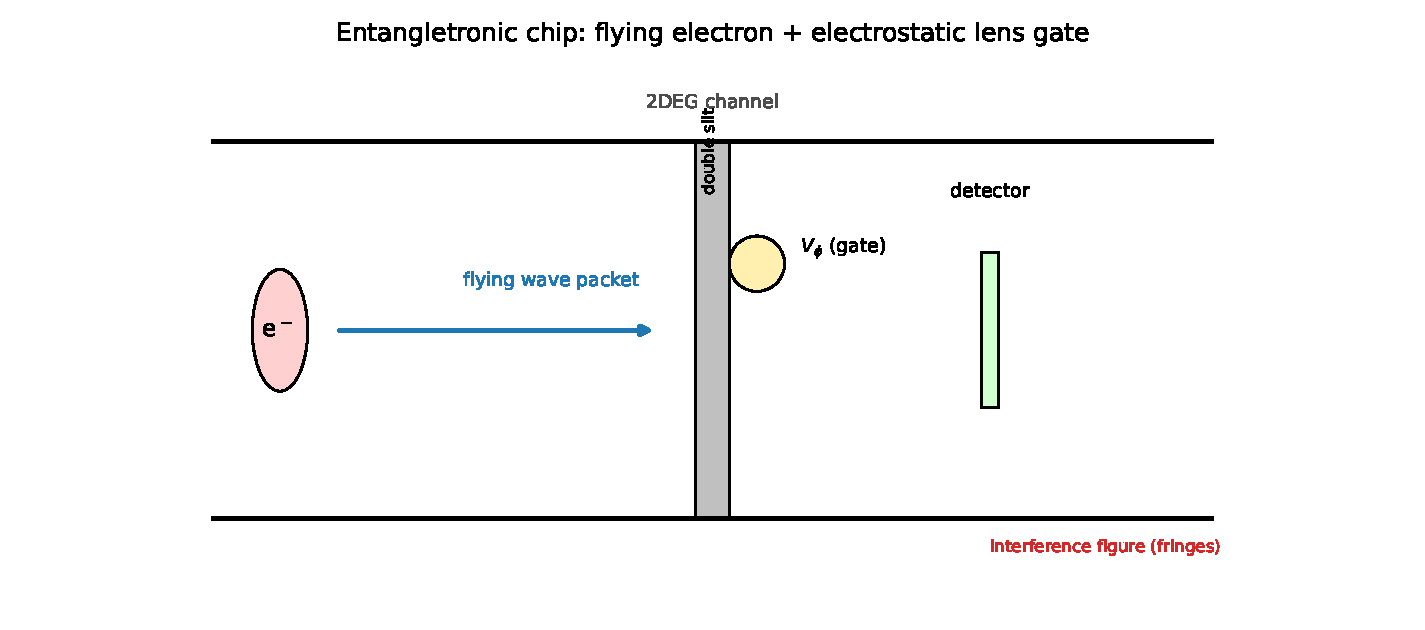
\includegraphics[width=0.85\linewidth]{../figures/fig1_architecture.pdf}
\caption{\textbf{Entangletronic device.} A single electron is launched into a
2DEG channel; a double-slit barrier splits the wave, a programmable phase lens
($V_\phi$) behind the upper slit imparts a phase shift in flight; a detector
reads the displaced interference figure.}
\label{fig:arch}
\end{figure}

\begin{figure}[t]
\centering
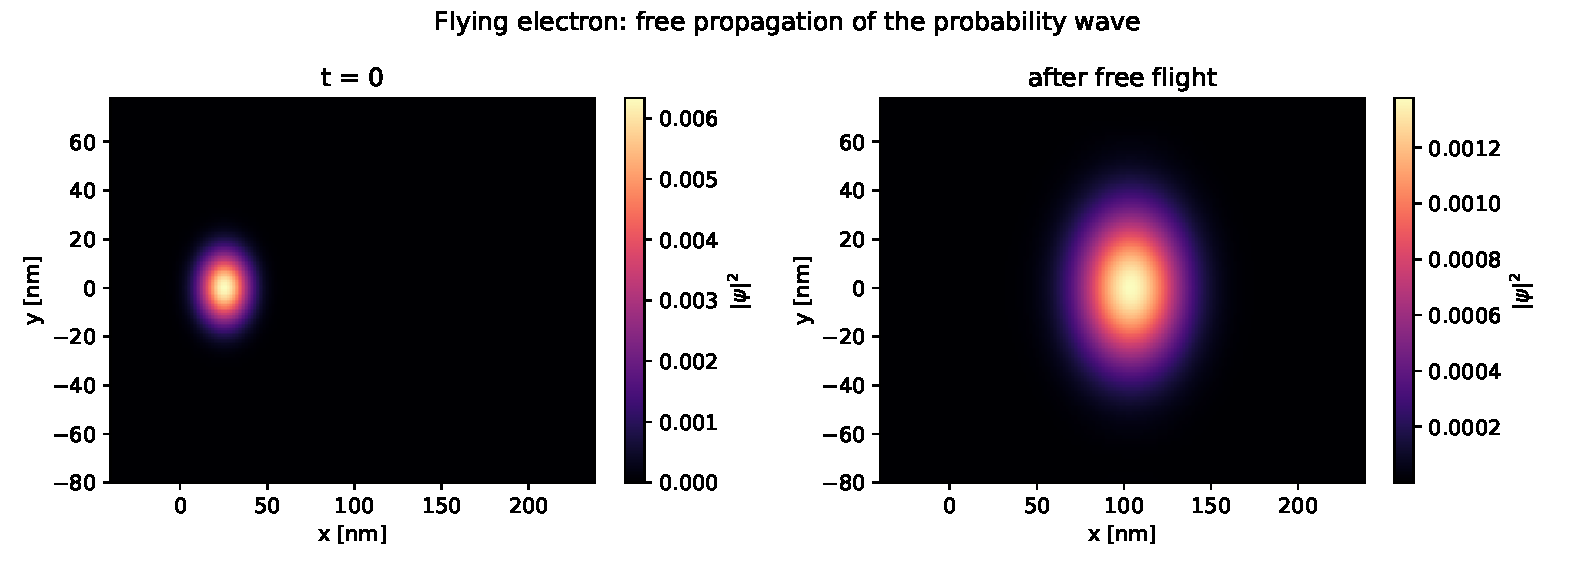
\includegraphics[width=0.95\linewidth]{../figures/fig2_free_propagation.pdf}
\caption{\textbf{Free flight of the flying electron.} $|\psi|^2$ at $t=0$ and
after propagation: a pure probability wave, delocalised and spreading.}
\label{fig:free}
\end{figure}

\begin{figure}[t]
\centering
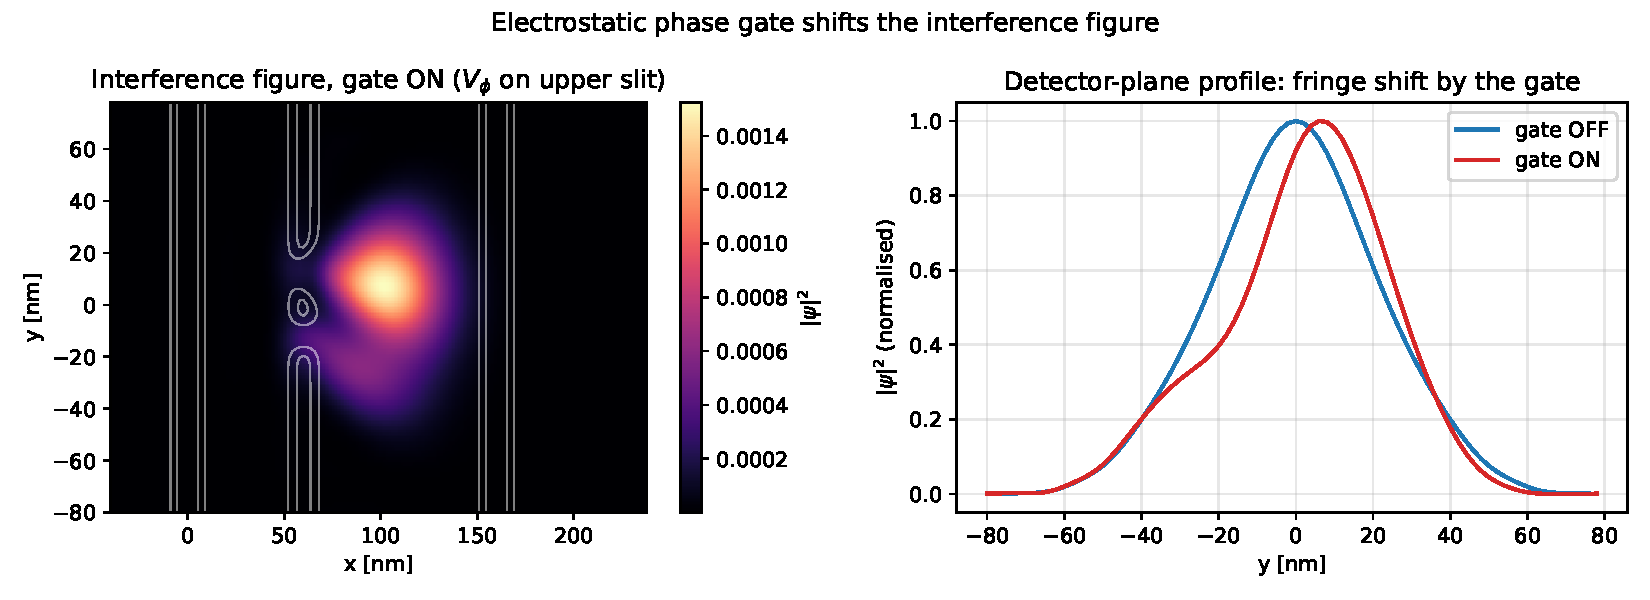
\includegraphics[width=0.98\linewidth]{../figures/fig3_interference.pdf}
\caption{\textbf{Interference figure and gate-induced shift.} Left: final
$|\psi|^2$ with the gate on (white contours: potential). Right: detector-plane
profile, gate off vs.\ gate on --- the fringe is displaced, the envelope is
not.}
\label{fig:interf}
\end{figure}

\begin{figure}[t]
\centering
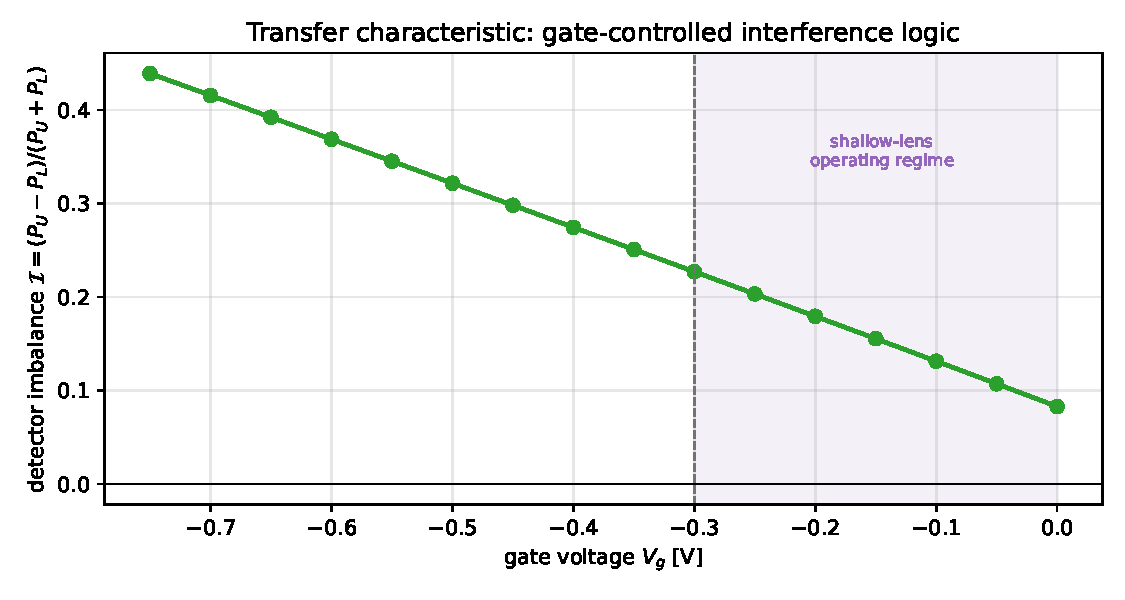
\includegraphics[width=0.72\linewidth]{../figures/fig4_transfer.pdf}
\caption{\textbf{Transfer characteristic.} Detector imbalance
Eq.~\eqref{eq:imb} vs.\ gate depth $\kphi$: linear with
$R^2 = 0.99997$. The gate is a linear transducer from voltage to
interference-logic.}
\label{fig:transfer}
\end{figure}

\begin{figure}[t]
\centering
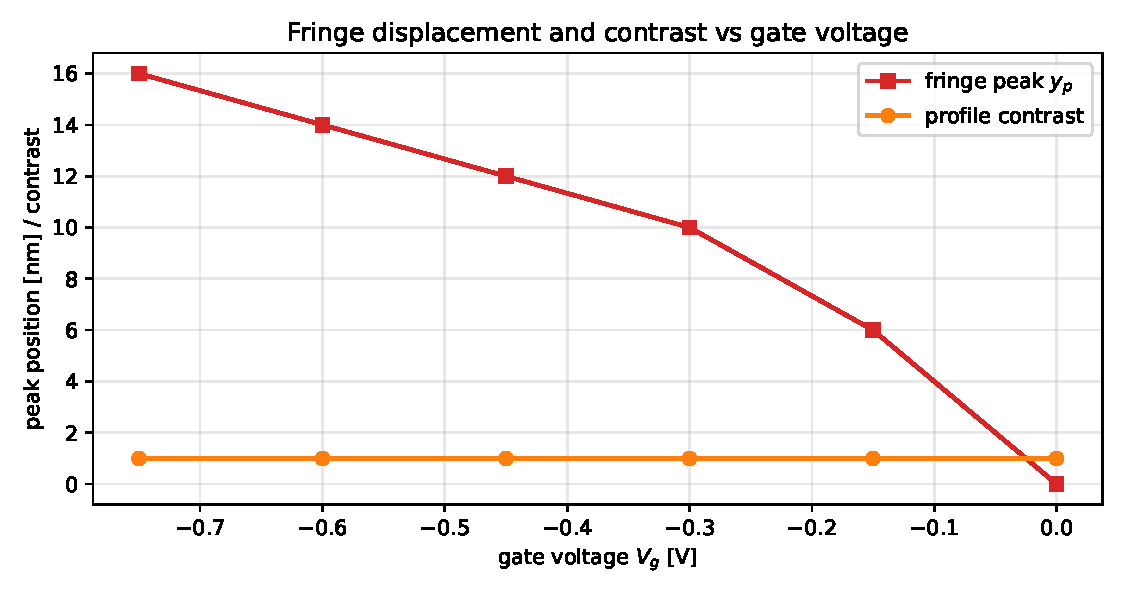
\includegraphics[width=0.72\linewidth]{../figures/fig5_fringe.pdf}
\caption{\textbf{Fringe displacement and contrast vs.\ gate.} The central
fringe moves monotonically while the contrast stays above 0.9: displacement
logic, not amplitude modulation.}
\label{fig:fringe}
\end{figure}

\end{document}
